\documentclass{llncs}
\usepackage{times}
\usepackage{graphicx}
\usepackage{latexsym}
\usepackage{multirow}
% \usepackage[scaled=.8]{beramono}
\usepackage[usenames,dvipsnames,svgnames,table]{xcolor}
\definecolor{light-gray}{gray}{0.95}
\usepackage[fleqn]{amsmath}
\usepackage{microtype}
\usepackage{verbatim}
\usepackage{paralist}
\usepackage{url}
\usepackage{listings}
\lstset{ %
   language=prolog,
%  frame=l,                     % adds a frame around the code
%   basicstyle=\footnotesize,  % use courier
   basicstyle=\footnotesize\ttfamily,	% use courier
   breaklines=true,
   xleftmargin=0.5em,
   xrightmargin=-0.5em,
   aboveskip=0.5em,
   belowskip=0.5em,
%  belowcaptionskip=5em,
   numbers=left,
   backgroundcolor=\color{light-gray},
   frame=single,
   framerule=0pt
}
\usepackage[usenames,dvipsnames]{xcolor}
\usepackage[disable]{todonotes}
\def\mnote#1{\todo[color=Goldenrod,size=\scriptsize]{Matt: #1}}
\def\jnote#1{\todo[color=CornflowerBlue,size=\scriptsize]{Julian: #1}}
\def\snote#1{\todo[color=WildStrawberry,size=\scriptsize]{Steve: #1}}

\setlength{\jot}{0pt}

% NOTES
% This is the fabula
% Syuzhet is all in the traversal
% Director could traverse nodes in a certain order
% Agents could abduce how to achieve narrative goals
% What we have here is also re-usable components

\begin{document}

% Long paper page limit: 12 pages

\title{Telling Non-Linear Stories with Interval Temporal Logic}

\author{Matt Thompson\inst{1} \and Steve Battle\inst{2} \and Julian Padget\inst{1} }
\institute{Department of Computer Science,\\
University of Bath, UK\\
\email{\{m.r.thompson,j.a.padget\}@bath.ac.uk}
\and
Dept. Computer Science and Creative Technologies,\\
University of the West of England, Bristol, UK\\
\email{steve.battle@uwe.ac.uk}}

\maketitle
\bibliographystyle{plain}


\begin{abstract}
Authoring a consistent interactive narrative is difficult without exhaustively specifying all possible deviations from the main path of a story. When automatically generating new story paths, it is important to be able to check these paths for consistency with the narrative world.
We present a method of describing the fabula of a story as a Kripke structure using Interval Temporal Logic, allowing the syuzhet to be expressed as a traversal of the structure. This allows the model checking of each possible telling of the narrative for consistency with the story world, as well as the ability to construct re-usable story components at different levels of abstraction. This is the first step towards building a fully checkable framework for building story components using modal logic.
\end{abstract}

\section{Introduction}
Agent-based approaches to interactive narrative generation must strike a balance between authorial control (writing a story structure), user agency and agent's actions (allowing characters to fill in the details of a story). One way to overcome this is to allow the author to describe the structure of a story in a way which constrains the available actions of the agents and user.
This introduces a problem: if there are multiple paths through a narrative (chosen by user interaction), how can an author describe alternative scenarios without explicitly writing out every single branch of the story? 

Narratologists such as Bal \cite{bal2009narratology} describe the construction of narrative in terms of \emph{fabula} and \emph{syuzhet}, where fabula is the sequence of events in a story as they occur in chronological order, and syuzhet is a subset of those events in the order in which they appear in the telling of the story. This means that a story can be modelled as a graph of events where the fabula is a straightforward traversal from a start node to an end node, and any syuzhet would be one of many possible ways of traversing the graph.
This simplifies our problem somewhat: if an author only needs to describe the events of a fabula, they only need create a graph of events occurring in chronological order. The user then experiences different stories by using different traversal methods. Similarly, agents would trigger events that cause the user's story to change state in a certain order.

This presents another problem, however. How can we check to make sure that the order of traversal for a syuzhet coheres to the rules of a story? For example, it could be possible that the murderer in a whodunit is revealed before the murder even takes place. Though this could be interesting in a more experimental narrative, most narratives would need to have some mechanism in place to prevent such an occurrence.
If the narrative is a non-linear or interactive one, then this problem is compounded further. In checking to see that a story traversal creates a coherent story, all possible branches and user decisions must be taken into account. Specifying which branches are correct, and in which order, would be time consuming if done by hand and expensive if all possibilities are searched with a computer program.

Riedl and Young \cite{riedl2010narrative} describe the problem as one of balancing \emph{author goals} and \emph{character goals}, introducing the technique of \emph{narrative mediation} to overcome it. This method represents the story as a partially ordered plan of (linear) events. An alternative plan is generated for any point at which the user can deviate from the original plan.
Narrative mediation has two strategies for dealing with possible narrative-breaking user interactions: \emph{accommodation}, where small changes to the narrative plan are made in order to incorporate the user's actions, and \emph{intervention}, which allows the user to perform (or seem to perform) the action, but does not allow it to have any effect on the narrative.
A drawback to this approach is the requirement for an initial analysis of the narrative plan to search for potentially story-breaking user actions. Every occurrence of this must be dealt with by another plan to accommodate or intervene with the action.

A wide variety of other approaches have been taken to address the same issue of balancing authorial and character control. A popular and effective one is to combine the use of a \emph{drama manager} with a Multi Agent System in order to regulate the actions of intelligent agents playing the parts of characters, telling them which actions to take in order to conform to a story. One of the first implementations of this approach was the Oz project at Carnegie Mellon University \cite{bates1992virtual}, ideas from which were later developed to become Mateas and Stern's \emph{Fa\c{c}ade} \cite{mateas2003faccade}.
Other approaches include the use of director agents \cite{lee2011learning}, reincorporation of player actions back into the narrative \cite{tomaszewski2011use} and mediation to prevent narrative-breaking actions \cite{robertson2013modelling}.

An approach that we have explored is to model the narrative as an institution of social norms, describing what the character agents are \emph{permitted} and \emph{obliged} to do at certain points in the story \cite{thompson-et-al:2015}. The advantage of this approach is that it merely suggests permitted actions to the agents, which have some degree of control over the actions they finally choose to carry out. For example, in an interactive narrative, a player could push a character so far that it causes them to deviate from the normal course of the story (albeit at some cost to the character agent). The goal of this approach is to permit greater agency for characters, while still encouraging them to perform within the constraints of a narrative.

In this paper we describe the use of modal logic, Interval Temporal Logic \cite{della2013interval}, and Kripke models \cite{kripke1963semantical} to describe the many paths which a narrative can take.

This approach is influenced by Marie-Laure Ryan's work describing possible worlds \cite{ryan1991possible} in the field of narratology. Ryan describes how, in the field of interactive narrative, the path one takes through a story is but one realisation of many possible story worlds. She asserts the link between possible worlds and modal logic, and Saul Kripke's work in particular. Taking this as inspiration, we formally develop these ideas in this paper.
The advantages of using Kripke structures to describe the story world are that it enables the checking of the world for inconsistencies, as well as the ability to create re-usable story components that can be combined in many different ways.

We begin with a description of the narrative formalism we use for our approach, Propp's Morphology of the Folktale \cite{propp1968morphology}, in section \ref{sec:propp}. The use of this formalism is demonstrated with an example from the \emph{Punch and Judy} story world in section \ref{sec:pjexample}. Section \ref{sec:propplogic} implements this example using Interval Temporal Logic and modal logic. Following this, Kripke models are then implemented using the LoTREC tableaux prover \cite{del2001lotrec} (section \ref{sec:kripke}).\mnote{Why do you want to use ITL \& Kripke models? What does this allow us to do?}
\mnote{Add relevance to digital storytelling. Logic allows richer capture of story structure}

\section{Propp's Morphology of the Folktale}\label{sec:propp}
To express story events in modal logic, we need some sort of formalisation for the analysis of the story~-- rather than an arbitrary selection of features~-- and so we look to narrative theory for inspiration. Instead of describing parts of the Punch and Judy story explicitly (such as `Punch is expected to hit the policeman in this scene'), it is desirable to describe scenes in a more abstract way using roles (`The villain fights the victim in this scene'). The use of more general story fragments allows us to reuse them in multiple scenes, or even in other stories.

Narratology, and structuralism in particular, supply such generalised building blocks for stories. Russian formalism is an early movement in narrative theory that sought to formalise the elements of narrative, and Vladimir Propp was a prominent figure in this school.  One outcome of this movement was Propp's 1928 formalism derived from the study of Russian folktales, \emph{The Morphology of the Folktale} \cite{propp1968morphology}, which is what we use to build a model to direct the course of the narrative.  In this formalism, Propp identifies recurring characters, which become roles, and motifs, which become action fragments, in Russian folklore, distilling them down to a concise syntax with which to describe stories. Propp's functional, event-driven style translates comfortably to an institution comprised of event-based norms. However, while these action fragments fit the Punch and Judy story adequately, we note that the role labels can sound rather awkward because of the apparent semantic import of the textual label.

In Propp's formalism, characters have \emph{roles}, such as \emph{hero}, \emph{villain}, \emph{dispatcher}, \emph{false hero}, and more. Characters performing a certain role are able to perform a subset of \emph{story moves}, which are actions that make the narrative progress. For example, the \emph{dispatcher} might send the \emph{hero} on a quest, or the \emph{victim} may issue an \emph{interdiction} to the \emph{villain}, which is then \emph{violated}.

Propp defines a total of 31 distinct story functions. Each function is given a number and symbol in order to create a succinct way of describing entire stories. Examples of such functions are:

\begin{compactitem}
  \item One of the members of a family absents himself from home: \emph{absentation}.
  \item An interdiction is addressed to the hero: \emph{interdiction}.
  \item The victim submits to deception and thereby unwittingly helps his enemy: \emph{complicity}.
  \item The villain causes harm or injury to a member of the family: \emph{villainy}.
\end{compactitem}

Each of these functions can vary in subtle ways. For example, the \emph{villainy} function can be realised as one of 19 distinct forms of villainous deed, including \emph{the villain abducts a person}, \emph{the villain seizes the daylight}, and \emph{the villain makes a threat of cannibalism}.
These functions are enacted by characters following certain roles. Each role (or \emph{dramatis persona} in Propp's definition) has a \emph{sphere of action} consisting of the functions that they are able to perform at any point in the story. Propp defines seven roles each of which has distinct spheres of action: \emph{villain}, \emph{donor}, \emph{helper}, \emph{princess}, \emph{dispatcher}, \emph{hero}, and \emph{false hero}.
In a typical story, one story function will follow another as the tale progresses in a sequential series of cause and effect. However, Propp's formalism does also allow for simultaneous story functions.

\subsection{Propp Example: Sausages and Crocodile Scene}\label{sec:pjexample}
To provide some context for Punch and Judy, since it is a peculiarly British phenomenon, although with Italian origins, we quote from Wikipedia:
\begin{quote}\small
Punch and Judy is a traditional, popular, and usually very violent puppet show featuring Mr Punch and his wife, Judy. The performance consists of a sequence of short scenes, each depicting an interaction between two characters, most typically Mr Punch and one other character (who usually falls victim to Mr. Punch's club). It is often associated with traditional British seaside culture.
The Punch and Judy show has roots in the 16th-century Italian commedia dell'arte. \\
\hfill{\footnotesize
\url{http://en.wikipedia.org/wiki/Punch_and_Judy}, retrieved 2015-05-06.}
\end{quote}

The common elements of Punch and Judy are easily described in terms of Propp's story functions. Here we pick one scene to use as an example: the scene where Punch battles a Crocodile in order to safeguard some sausages.  In this scene, Joey the clown (our narrator) asks Punch to guard the sausages. Once Joey has left the stage, a Crocodile appears and eats the sausages. Punch fights with the Crocodile, but it escapes. Joey then returns to find that his sausages are gone.
The corresponding story functions are:
\begin{enumerate}
  \item Joey tells Punch to look after the sausages (\emph{interdiction}).
  \item Joey has some reservations, but decides to trust Punch (\emph{complicity}).
  \item Joey gives the sausages to Punch (\emph{provision or receipt of a magical agent}).
  \item Joey leaves the stage (\emph{absentation}).
  \item A Crocodile enters the stage and eats the sausages (\emph{violation}).
  \item Punch fights with the Crocodile (\emph{struggle}).
  \item Joey returns to find that the sausages are gone (\emph{return}).
\end{enumerate}

Some story functions map to Punch and Judy better than others (for example, it is debatable as to whether or not the sausages can be considered a ``magical agent''), but Propp's formalism seems well suited to Punch and Judy for the most part. The advantage of using Propp for the Punch and Judy story domain is that the story function concept maps well to the idea of internal events in institutional models.

\section{Combining Interval Temporal Logic and Modal Logic for Propp}\label{sec:propplogic}
\mnote{Put in definitions as a footnote, Cyrillic if you want}
Narrative construction can be described using two terms: \emph{fabula} and \emph{syuzhet}. Fabula is the events of the story as they occur in chronological order, but syuzhet refers to those events as they are ordered in the story's telling. Fabula describes one event following another, but syuzhet could describe events occuring out of order, branching sequences and events that occur at the same time.

The challenge faced here is how to find a way of not only describing the syuzhet of one story, but of all possible stories and paths through a story in a narrative world.

\subsection{Modal Logic}
Modal logic extends classical propositional and predicate logic with modalities, which are operators that qualify a statement. For example, rather than simply stating `The Crocodile eats the sausages', we could instead say ``the Crocodile sometimes eats the sausages'', or ``it's possible that the Crocodile eats the sausages''.
Classic modal logic deals with \emph{alethic modality}, which describes whether a statement is \emph{possible} or \emph{necessary}. This is implemented using unary operators to qualify statements. For example, $\Diamond P$ states that $P$ is possible and $\Box P$ states that $P$ is necessary.
Naturally, we can use modalities beyond just possibility and necessity. In order to describe the syuzhet of a story, we need to be able to make statements such as ``The Crocodile eats the sausages at the beginning of the scene'', and ``Punch kills the baby while before his wife returns''. For this, we turn to \emph{temporal logic}.

\mnote{Why use modal logic for possible worlds?}

\subsection{Temporal Logics}
Arthur Prior is the first to employ modal logic as a way of describing sequences of time in his 1957 work \emph{Time and Modality} \cite{prior2003time}. Here he uses just two modal operators, $P$ and $F$, representing \emph{some time in the past} and \emph{some time in the future} respectively.
Hans Kamp adds two extra operators to Prior's logic, \emph{Since} and \emph{Until}, in his 1968 thesis \cite{kamp1968tense}, enabling it to describe spans of time in addition to the ordering of temporal events.
As Kripke later points out to Prior, this model lacks the expressiveness needed to describe all possible sequences of events. One major shortcoming is its restriction to describing only \emph{linear} events. 

Linear Temporal Logic (LTL), though still limited to the description of linear sequences of events, is an evolution of the work done by Prior and Kamp. Proposed by Amir Pnueli in 1977 \cite{pnueli1977temporal}, its original use is for the formal verification of computer programs.
Computational Tree Logic (CTL) \cite{ben1983temporal} is similar to LTL, but allows for the representation of non-linear time through the allowance of branches. Through CTL it is possible to describe several alternative pathways through time, though only one may ever be actualised. Like LTL, its original purpose is for formal verification of software, and in model checkers.
Both CTL and LTL are subsets of CTL* (Computational Tree Logic) \cite{emerson1986sometimes}, which can both describe both multiple branches of temporal paths and their durations. CTL* formulae must refer to a specific Kripke structure, however (a description of Kripke structures appears in section \ref{sec:kripke}).

\subsubsection{Interval Temporal Logic}
In order to model fabula with modal logic, we employ Interval Temporal Logic (ITL), composed of the temporal intervals defined by Allen \cite{allen1983maintaining} and developed into modal operators by Halpern and Shoham \cite{halpern1991propositional}. This allows the expressiveness necessary to describe branching, parallel and nested paths through stories.

In most temporal logics (such as CTL* and its subsets), fixed \emph{time points} without duration are the basic unit of time. However, this can make it difficult to reason about the \emph{duration} of events that occur over a period of time. Temporal Interval Logic tackles this problem through the use of \emph{time intervals} or \emph{periods} as the basic temporal unit.

The version of ITL used here is that described by Della Monica et al. in their overview paper \cite{della2013interval}. Figure \ref{fig:itl} lists the temporal intervals described by Allen, along with their modal operator equivalents in \emph{Halpern-Shoham logic}.

The operators defined by Halpern and Shoham are (a bar over an operator denotes its inverse):

\begin{itemize}
\item $\langle L \rangle / \langle \overline{L} \rangle$ (Later): The interval occurs at some point after another interval.
\item $\langle A \rangle / \langle \overline{A} \rangle$ (After): The interval occurs immediately after another interval.
\item $\langle O \rangle / \langle \overline{O} \rangle$ (Overlaps): The interval occurs both during and before or after another interval.
\item $\langle E \rangle / \langle \overline{E} \rangle$ (Ends): The interval ends at exactly the same time as another interval.
\item $\langle D \rangle / \langle \overline{D} \rangle$ (During): The interval both starts and ends inside the duration of another interval.
\item $\langle B \rangle / \langle \overline{B} \rangle$ (Begins): The interval begins at exactly the same time as another interval.
\end{itemize}
\mnote{Put a detailed explanation in here.}

\mnote{Try to get higher res table or recreate it myself.}

\begin{figure}[!t]\label{fig:itl}
  \centering
    \centerline{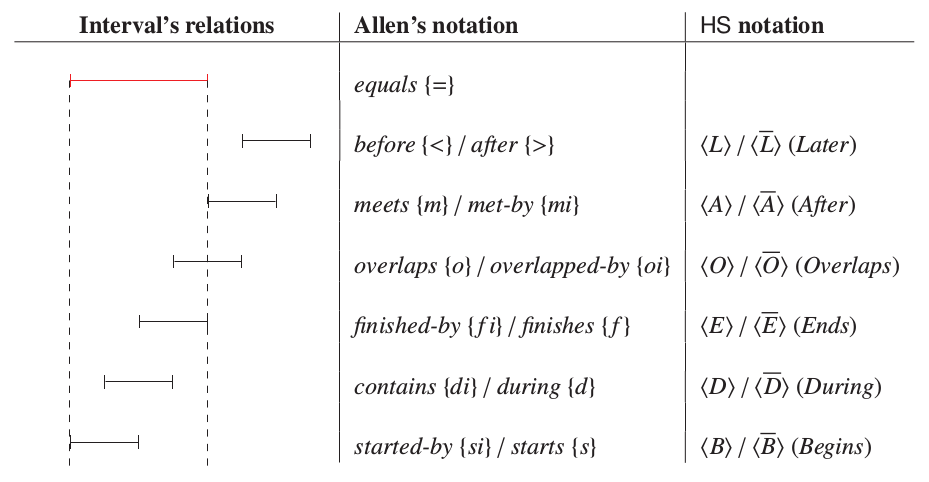
\includegraphics[height=2.5in]{itl.png}}
  \caption{Operators in the Interval Temporal Logic (taken from \cite{della2013interval})}
\end{figure}

\subsection{Propp Example with Punch and Judy}

In this example, we combine Halpern and Shoham's temporal operators with the possibility ($\Diamond$) and necessity ($\Box$) operators of modal logic. We follow the convention of writing possibility operators inside angle brackets: $\langle \, \rangle$ and necessity operators within square brackets: $[ \, ]$.

This example shows the ``sausages'' scene described in section \ref{sec:pjexample}, consisting of a set of situations $S$, containing Propp story functions $P$. The interval temporal logic operators used in this example are the set $T$. Figure \ref{fig:operators} shows the modal operators we use. $A, B$ and $C$ in formula \ref{eq:story} are variables that represent the characters and objects that appear in the story.

\begin{figure}
\begin{align}
    S &= \{S_0, S_1, S_2, S_{3a}, S_{3a_1}, S_4, S_{3b}, S_{3b_1}, S_4, S_5\}\\
    P &= \{\mathtt{interdiction(A, B, C), absentation(A), struggle(A, B),}\nonumber\\
  &\qquad\qquad\mathtt{victory(A), villainy(A, B), violation(A, B), return(A)}\}\label{eq:story}\\
  T &= \{D, \overline{D}, O, \overline{O}, A, \overline{A}, B, \overline{B}, L, \overline{L}, E, \overline{E}\}
\end{align}
\caption{Modal operators}\label{fig:operators}
\end{figure}
Hybrid logics allow worlds, time intervals, to be named. The hybrid logic nominal operator allows specific times to be uniquely referenced, allowing a logic to talk about specific states such as $S_0..S_5$. The nominal proposition is true of one specific time interval such that any two worlds with the same name represent co-extensive intervals of time. Anything true of one is true of the other.
We also make use of a nominal modal operator so that it is possible to make assertions about these named worlds, ``It is necessary that in state $S_1$ Joey absents himself.'' This technique enables us to associate story functions with specific, named intervals.
We use hybrid logic to identify nodes using the \emph{nominal} operator, shown as $@$. The nominal operator adds the capability of referring to possible worlds in formulas. In this way, each possible state of a system can be labelled and referenced from other states. As seen in figure \ref{fig:lotrec}, each nominal node must have its own name as a relation leading back to the root node, in order to be linked to and referred from the other nodes.
We can combine this with the Interval Temporal Logic to make statements such as ``An absentation starts with state $@S_1$ and end with state $@S_5$.'' (formula \ref{eq:absentation}).
Figure \ref{fig:situations} describes the full sausages scene from Punch and Judy using the time intervals shown in figure \ref{fig:durations}.

\begin{figure}[!t]
  \centering
    \centerline{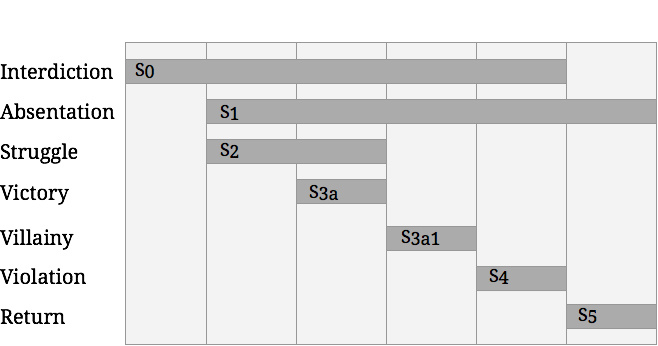
\includegraphics[width=0.9\textwidth]{durations.png}}
  \caption{Timings of the story functions in the sausages scene}\label{fig:durations}
\end{figure}
\begin{figure}[]
\begin{align}
  &S_{0} \land \mathit{interdiction(Joey, Punch, Sausages)} \land\nonumber\\
  &\qquad\qquad\qquad\qquad\qquad\langle B \rangle @S_{1} \land \langle E \rangle @S_{4} \land \langle A \rangle @S_{5}\label{eq:interdiction}\\
  &[@S_{1}] \mathit{absentation(Joey)} \land \langle A \rangle @S_{2}\label{eq:absentation}\\
  &[@S_{2}] \mathit{struggle(Punch, Crocodile)} \land \langle E \rangle (@S_{3a} \lor @S_{3b})\label{eq:struggle}\\
  &[@S_{3a}] \mathit{victory(Crocodile)} \land \langle A \rangle @S_{3a_1}\\
  &[@S_{3a_1}] \mathit{villainy(Crocodile, Sausages)} \land \langle E \rangle @S_{4}\\
  &[@S_{3b}] \mathit{victory(Punch)} \land \langle A \rangle @S_{3b_1}\\
  &[@S_{3b_1}] \mathit{villainy(Punch, Sausages)} \land \langle E \rangle @S_{4}\\
  &[@S_{4}] \mathit{violation(Punch, Sausages)}\\
  &[@S_{5}] \mathit{return(Joey)}
\end{align}
\caption{Sausages scene with nominals and Interval Temporal Logic}\label{fig:situations}
\end{figure}


One notable feature of this approach is that it enables the building of reusable story components. For example, we have said that an interdiction must begin with an absentation and ends with a violation (formula \ref{eq:interdiction}). This pattern can be reused in different stories, or several times in the same story. Additionally, it allows for the abstraction and combination of story components in a more expressive way than Propp's original story functions. This is because Propp only describes narrative events at one level of abstraction. For example, he describes stories as a series of events containing an interdiction followed by an absentation, followed by a violation. But there is no mechanism for combining these three functions into a higher-level component (which could be called ``Don't do that, or else!'', for example). Our approach makes such abstraction and recombination possible.

\section{Describing Punch and Judy with Kripke Structures}\label{sec:kripke}
\begin{figure}[!t]
  \centering
    \centerline{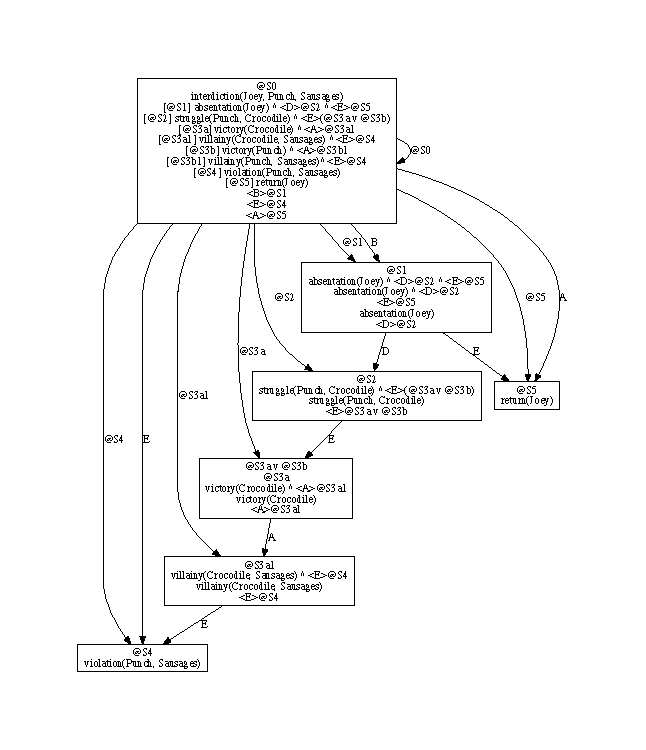
\includegraphics[width=0.9\textwidth]{crocmodel.pdf}}
  \caption{One model from the sausages scene in LoTREC}\label{fig:lotrec}
\end{figure}

We use Kripke structures \cite{kripke1963semantical} as a method of interpreting the combination of modal logic with Interval Temporal Logic. A Kripke structure is a graph, the nodes of which represent a possible world consisting of a set of assertions, and the edges of which are the accessibility relations between worlds.

\subsection{LoTREC}
% Read the book
In order to build and visualise the Kripke structures, we use LoTREC \cite{del2001lotrec}, a generic tableaux prover for modal and description logics. It allows the user to build up Kripke models using a domain specific language and display those models in the form of a graph diagram.
LoTREC uses the tableau method for model checking. This method checks whether or not its input is satisfiable by attempting to build a model for it. If the model construction fails, then the input is unsatisfiable.
Building models in LoTREC consists of defining \emph{connectors}, \emph{rules} and \emph{strategies}. Connectors are the logical operators used in formulas, rules are the instructions LoTREC needs to expand them into new nodes and edges and strategies are ways of combining rules in order to form models.
LoTREC takes an initial set of formulas as input and expands each formula into its components. These formulas are input using a simple prefix notation domain specific language consisting of operators and arguments, described in the LoTREC instruction book \emph{Kripke's Worlds} \cite{gasquet2013kripke}.
In the expansion, if a $[\,]$ (necessary) operator is encountered, then the formulas that serve as its argument are propagated across to all subsequent nodes. In the case of a $\langle \, \rangle$ (possibility) operator, a new node (possible world) is created containing its arguments. In both cases, binary operators can be used where one argument is located inside the square or angle brackets. In these cases, the argument inside the brackets is the accessibility relation, and is used to label the edges leading to the subsequent nodes.
In the case of a disjunction ($\lor$) operator, the current model is copied in its entirety and extended with one of the operator's arguments. The other argument is added onto the current model. This is an important way of creating alternative routes through the narrative, all of which can be checked for consistency.

\subsection{The Sausages Scene in LoTREC}
The narrative is captured as a system of interval temporal logic assertions over story functions. The  assertions are interpreted using a tableaux reasoner by unpacking them to form a Kripke structure.
Using the initial formulas from figure \ref{fig:situations} as input, figure \ref{fig:lotrec} shows the model for the case where Punch wins the fight with the Crocodile. One other model exists in this scenario, in which the Crocodile is instead the victor.

The example in figure \ref{fig:lotrec} describes the fabula of a branching story, where either Punch or the Crocodile may win the fight for the sausages. This corresponds to the disjunction in figure \ref{fig:situations}, formula \ref{eq:struggle}. This leads to the creation of two models: the one in which the Crocodile wins and then goes on to eat the sausages (situation $@S_{3a}$), and the one in which Punch wins (situation $@S_{3b}$).
Using a breadth first strategy like LoTREC we would build all models simultaneously. This enables them to be checked for internal consistency, eliminating potentially impossible temporal arrangements. For example, no interval may come after or later than itself.

The first node contains the logical description of the story, which is then unpacked into subsequent nodes. It starts with the initial situation, $S_0$, which contains an interdiction: $\mathit{interdiction(Joey, Punch, Sausages)}$, where Joey tells Punch to look after the sausages. The other situations, $S_1$ to $S_5$ are listed using the necessity operator, with their accessibility relations being each situation's nominal operator (such as $@S_1$). This means that these situations are all created as new nodes, linked to the root node using their nominal accessibility relation, and so can be referred to later using the nominal operator. In this way, situations can refer to other situations.

For example, in Propp's formalism, an interdiction must begin with the absentation of a character and end with the interdiction's violation. For this reason, the initial situation is connected to $@S_1$, ($\mathit{absentation(Joey)}$), with the $\langle B \rangle$ (begins) accessibility relation and to $@S_4$, ($\mathit{violation(Punch, Sausages)}$), with the $\langle E \rangle$ (ends) accessibility relation. As other situations are unpacked into nodes, they are linked to other situations in the same way. An example of this is shown in $S_1$, the absentation, which must end with Joey's return, $S_5$, and during which a struggle must occur ($S_2$). As the formulas inside $S_1$ are unpacked, $S_1$ is linked to the other situations with the appropriate temporal accessibility relations. This is all made possible with the hybrid logic, which allows nodes to be referred to by name and linked to.

By describing situations that are linked together with temporal relations, we can build narratives and check them as we go. If a narrative is inconsistent in some way (by stating that a character is both dead and alive, for example), then the model will be unsatisfiable. This is useful for ensuring the construction of consistent narratives.

Additionally, every time a story has the possibility of branching off, the model for each new branch can be checked to see if it is viable in the narrative world. This means that rather than relying on an author to write out each branch of a story, they can be generated automatically from a story description and checked for inconsistencies.

As mentioned previously, the combination of Interval Temporal Logic and a narrative formalism such as Propp's allows us to create abstracted story components. For example, we have described the interdiction as being started by an absentation and ended with a violation. This pattern can be called the ``interdiction pattern'', and so can be easily reused in other narratives.

The use of LoTREC has shown the utility of being able to visualise a branching narrative in its entirety. This suggests that our method enables the visual authoring of interactive narratives by non-technical creators. Rather than having to type in computer code, or logical formulas, a visual tool could be developed to create logically consistent narrative worlds.

\section{Conclusions and Future Work}
This paper demonstrates the use of interval temporal logic for the construction of non-linear narratives. The advantages of this approach are that it enables an author to create re-usable story components at various levels of abstraction. It also allows for the model-checking of a proposed narrative of subset of a narrative to see if it fits with an author's model of a narrative world.

Using this method, the fabula of a story could be laid out in the original model, with the syuzhet emerging from different ways of traversing the graph. By using interval temporal logic, we ensure that the nodes of the graph can only be traversed in certain orders, thus ensuring the coherence of the narrative.

This approach for describing narrative has many potential real-world uses. One obvious use would be for computer game narratives, but it could also be used to describe a repeatable training scenario, and the possible choices available to a user at any point during the simulation.

This work is the first step towards creating a modal-logic based method for story description with reusable narrative motifs. In this instance we have used Propp as our narrative formalism, but this approach allows for the description of story components at different levels of abstraction. For example, the ``Hero's journey'' story type could be composed of a ``Call to adventure'' component, followed by a ``Suffering of hardship'' component, then a ``Achievement of victory'' component. These components can then be further sub-divided into smaller and smaller story components. Depending on the level of control an author desires, story components could be left entirely for character agents to act out (based on given pre and postconditions), but the amount of control the characters have over the story would depend on the level of abstraction of the story component they are acting out.

From this point, we hope to explore alternative narrative formalisms outside of Propp. Though Propp works well for simple examples, modern media use story motifs that require some stretching of his story functions. We also intend to take our approach outside of the confines of the LoTREC software, into a live interactive storytelling program. In this way, we will be able to evaluate the effectiveness of our approach both in terms of story authoring and believability for the player.

\bibliography{icids}

\end{document}

